\documentclass[xetex, svgnames, 12pt]{scrartcl}
\usepackage{xltxtra}
\usepackage{polyglossia}
\usepackage{xcolor,color}
\usepackage{xeCJK}
\usepackage{multirow}
\usepackage{placeins}
\usepackage{array,covington}
\usepackage{tabu,booktabs}
\usepackage{array} 
\usepackage{multirow}
\usepackage{textcomp}
\usepackage{tabularx,booktabs} 
\usepackage{color,soul}
\newfontfamily\sil{DejaVu Sans}
\newfontfamily\burm{Padauk}
\newfontfamily\hana{Noto Sans CJK SC}

\usepackage[normalem]{ulem}
%\setCJKmainfont{AR PL UMing TW}
\newcommand\comment[1]{\textcolor{red}{#1}}
%\usepackage[left=2cm,right=2cm,top=3cm,bottom=3cm]{geometry}
\usepackage[left=2.5cm, right=2.5cm, top=3cm, bottom=3cm]{geometry}
\newcommand\commentmattis[1]{\textcolor{DarkGreen}{[#1] \#lingulist}}
\newcommand\commentnathan[1]{\textcolor{blue}{[#1] \#nh36}}
\usepackage[round]{natbib}
\usepackage[
    colorlinks,
    urlcolor=black,
    linkcolor=black,
    citecolor=CornflowerBlue,
    filecolor=black,
    pagecolor=black,
    linktocpage=true,
    %dvipdfm
    ]{hyperref}
\usepackage[]{tikz}
\graphicspath{{images/}{../images/}}
\usepackage{setspace}

\usetikzlibrary{calc,arrows,positioning,shapes}

\newcommand{\SET}[1]  {\ensuremath{\mathcal{#1}}}
\newcommand{\MAT}[1]  {\ensuremath{\boldsymbol{#1}}}
\newcommand{\VEC}[1]  {\ensuremath{\boldsymbol{#1}}}
\newcommand{\Video}{\SET{V}}
\newcommand{\video}{\VEC{f}}
\newcommand{\track}{x}
\newcommand{\Track}{\SET T}
\newcommand{\LMs}{\SET L}
\newcommand{\lm}{l}
\newcommand{\PosE}{\SET P}
\newcommand{\posE}{\VEC p}
\newcommand{\negE}{\VEC n}
\newcommand{\NegE}{\SET N}
\newcommand{\Occluded}{\SET O}
\newcommand{\occluded}{o}
%\definecolor{amazongreen}{cmyk}{0.83,0.24,0,0.12}
\definecolor{blue}{rgb}{0.0, 0.0, 0.55}
\definecolor{green}{rgb}{0.0, 0.5, 0.0}
\definecolor{red}{rgb}{0.75, 0.0, 0.2}
\definecolor{violet}{RGB}{153,153,255}
\definecolor{antiquewhite}{rgb}{0.98, 0.92, 0.84}
\definecolor{amazongreen}{RGB}{0,153,153}

\title{Asia.bib master project}
\author{Asia.bib}

\begin{document}
\maketitle

This is the \verb=asia.bib= master project. In order to update \verb=asia.bib=, please do as follows.

\begin{itemize}
\item Download \verb=asia.bib=, change it, and reupload it here.
\item Make sure that this Overleaf V2 project compiles without errors -- this file shows every single item in \verb=asia.bib= so that we can be sure that the compilation is not broken.
\item Push the changes back into the GitHub project, so that we can keep a tracklog of the changes: click on the left-top ``Menu'', then ``Sync -- GitHub'', then click on this button:
\begin{center}

\includegraphics[width=10.5em]{a.png}
\end{center}
\item Pull the changes in the Overleaf project where the bibliography item is needed:
\begin{center}
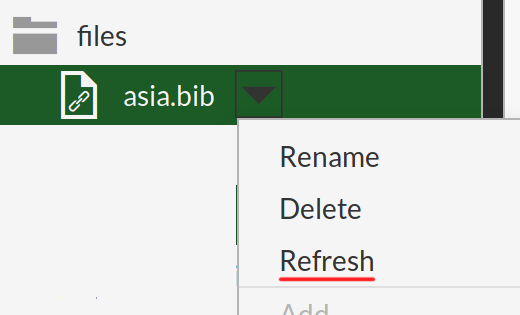
\includegraphics[width=15em]{refresh.png}
\end{center}
\end{itemize}

\nocite{*} % Shows the bibliography items here

\bibliographystyle{plainnat}
\bibliography{asia.bib}

\end{document}